% Numerical Computing II
% Homework 20
% Properties of Eigenvalues and Eigenvectors
% 4/5/20
% 20.1, 20.2, 20.4, 20.5, 20.6, 20.7

\documentclass[11pt]{article}
\usepackage{listings}
\usepackage[fleqn]{amsmath}
\usepackage{graphicx}
\begin{document}         
\lstset{language=Matlab,numbers=left,frame=single,breaklines=true,morecomment=[l]{//}}
% Start your text
\newcommand{\makehomework}[2]%
{\begin{center}%
	\Huge #1\\%
	\Large #2\\%
	Marty Fuhry\\%
	\today%
\end{center}}
\makehomework{Numerical Computing II}{Homework 20: Properties of Eigenvalues and Eigenvectors}

\section*{Exercise 20.1}
To show that an $n \times n$ matrix $A$ with $n$ distinct eigenvectors has $n$ linearly independent eigenvectors, we assume the contrary.
That is, assume that some eigenvector of $A$, $v_i$ can be represented as a linear combination of the other
eigenvectors. Then,

\begin{flalign*}
    0 &= c_1 v_1 + \cdots + c_i v_i + \cdots + c_n v_n\\
      &= A (c_1 v_1 + \cdots + c_i v_i + \cdots + c_n v_n)\\
      &= c_1 A v_1 + \cdots + c_i A v_i + \cdots + c_n A v_n\\
      &= c_1 \lambda_1 v_1 + \cdots + c_i \lambda_i + \cdots + c_n \lambda_n v_n.
\end{flalign*}
We multiply the first line here with $\lambda_i$ to obtain
\begin{flalign*}
    0 &= c_1 \lambda_i v_1 + \cdots + c_i \lambda_i v_i + \cdots + c_n \lambda_i v_n.
\end{flalign*}
Then, we can subtract this equation from the second one to remove the $c_i \lambda_i v_i$ term completely
and maintain a constant $0$ as the sum.
\begin{flalign*}
     0 &= c_1 (\lambda_1 - \lambda_i) v_1 + \cdots + c_i (\lambda_i - \lambda_i) v_i + \cdots + c_n (\lambda_n - \lambda_i) v_n.\\
      &= c_1 (\lambda_1 - \lambda_i) v_1 + \cdots + 0 + \cdots + c_n (\lambda_n - \lambda_i) v_n.
\end{flalign*}
But each $\lambda_j \neq \lambda_i$, so they cannot evaluate to $0$. 
$\Rightarrow\Leftarrow$


\section*{Exercise 20.2}

\section*{Exercise 20.4}
\section*{Exercise 20.5}
\section*{Exercise 20.6}
\section*{Exercise 20.7}
% 20.1, 20.2, 20.4, 20.5, 20.6, 20.7
% Import Program 
%\lstinputlisting{problem_17_1.m}

% Import Graph
%\begin{center}
%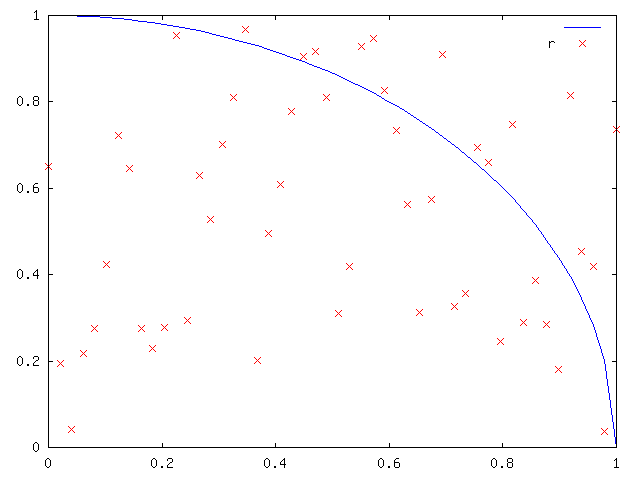
\includegraphics[scale=0.5]{problem_17_1_graph.png}
%\end{center}

% Stop your text
\end{document}
